\documentclass[border=1pt]{standalone}

\usepackage{amssymb}
\usepackage{tikz}
\usetikzlibrary{intersections}

\newcommand{\PP}{\mathbb P}

% colors
\definecolor{page}{HTML}{b8e5fe}
\definecolor{sheet}{HTML}{d6edfe}
%\definecolor{outline}{rgb}{0.6, 0.75, 0.9}
%\definecolor{outline}{rgb}{0.4, 0.5, 0.6}
\definecolor{outline}{rgb}{0.3, 0.375, 0.45}

\newcommand{\hiddenline}{black!30!sheet}
\newcommand{\spot}{ellipse [x radius=6.4pt, y radius=4.5pt, rotate=4]}

\begin{document}
    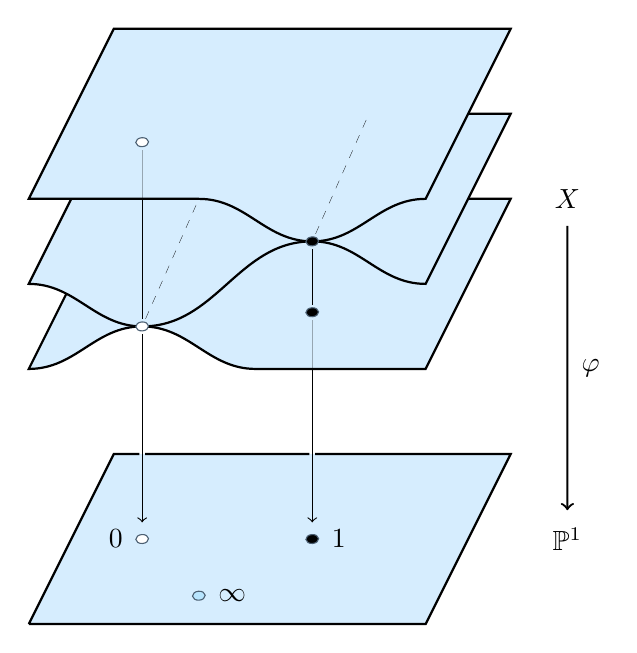
\begin{tikzpicture}[scale=.36]
      % sheet fills
      \begin{scope}[sheet]
      \fill (0,9) to[out=0,in=-180] (4,10.5) to[out=0,in=-180] (8,9) -- (14,9) -- (17,15) -- (3,15) -- cycle;
      \fill (0,12) to[out=0,in=-180] (4,10.5) to[out=0,in=-180] (10,13.5) to[out=0,in=-180] (14,12) -- (17,18) -- (3,18) -- cycle;
      \fill (0, 15) -- (6,15) to[out=0,in=-180] (10,13.5) to[out=0,in=-180] (14,15) -- (17,21) -- (3,21) -- cycle;
      \end{scope}
      
      % base
      \fill[fill=sheet] (0,0) -- (14,0) -- (17,6) -- (3,6) -- (0,0);
      \draw[thick] (0,0) -- (14,0) -- (17,6) -- (10.1, 6) (9.9, 6) -- (4.1, 6) (3.9, 6) -- (3,6) -- (0,0);
      
      % branching
      \begin{scope}[ultra thin, dashed, shorten <=3pt]
      \draw (4,10.5)--(6,15);
      \draw (10,13.5)--(12,18);
      \end{scope}
      
      % projection to 0
      \draw[<-, black, shorten <=6pt, shorten >=2.7pt] (4,3) -- (4,10.5);
      \draw[black, shorten <=2.7pt] (4,10.5) -- (4,15);
      \draw[\hiddenline, thin, shorten >=2.7pt] (4,15) -- (4,17);
      
      % projection to 1
      \draw[<-, black, thin, shorten <=6pt] (10,3) -- (10,9);
      \draw[\hiddenline, thin, shorten >=2.7pt] (10,9) -- (10,11);
      \draw[black, thin, shorten <=2.7pt, shorten >=2.7pt] (10,11) -- (10,13.5);
      
      % sheet outlines
      % we can't intersect with the sheet 2 fill because the intersections library
      % can't handle parallel lines
      % https://tex.stackexchange.com/a/581465/6934
      \path[name path=seg-2] (0,12) to[out=0,in=-180] (4,10.5);
      \path[name path=seg-1] (3,15) -- (0,9);
      \draw[thick, name intersections={of=seg-2 and seg-1}] (intersection-1) -- (0,9) to[out=0,in=-180] (4,10.5) to[out=0,in=-180] (8,9) -- (14,9) -- (17,15) -- (15.5,15);
      % sheet 2 outline
      \draw[thick] (1.5,15) -- (0,12) to[out=0,in=-180] (4,10.5) to[out=0,in=-180] (10,13.5) to[out=0,in=-180] (14,12) -- (17,18) -- (15.5,18);
      % sheet 3 outline
      \draw[thick] (0, 15) -- (6,15) to[out=0,in=-180] (10,13.5) to[out=0,in=-180] (14,15) -- (17,21) -- (3,21) -- cycle;
      % zero
      \draw[outline, fill=white] (4,3) \spot;
      \node at (4,3) [label=left:$0$] {};
      \draw[outline, fill=white] (4,10.5) \spot;
      \draw[outline, fill=white] (4,17) \spot;
      
      % one
      \draw[outline, fill=black] (10,3) \spot;
      \node at (10,3) [label=right:$1$] {};
      \draw[outline, fill=black] (10,11) \spot;
      \draw[outline, fill=black] (10,13.5) \spot;
      
      % infinity
      \draw[outline, fill=page] (6,1) \spot;
      \node at (6,1) [label=right:$\infty$] {};
      
      % morphism label
      \node[outer sep=3pt] (coverlabel) at (19,15) {$X$};
      \node[outer sep=3pt] (baselabel) at (19,3) {$\PP^1$};
      \draw[black,->,thick] (coverlabel) to node[right=0.5mm]{$\varphi$} (baselabel);
    \end{tikzpicture}
\end{document}
